\documentclass[xetex]{beamer}
% \setbeameroption{show only notes}
\usefonttheme[onlymath]{serif}
\usefonttheme{serif}
\usepackage{tikz}
\usepackage{graphicx}
\usetheme{metropolis}
\usepackage{lmodern}
\usepackage{amsmath}
\usepackage{mathrsfs}
\usepackage{pdfpages}
\usepackage[backend=biber, style=science]{biblatex}
\addbibresource{/Users/fergusbarratt/bibTex/library.bib}
\graphicspath{ {../../../Images/Presentation/} }
%----------------------------------------------------------------------
\title{The Dissipative-Driven Jaynes-Cummings System}
\subtitle{The dispersive regime and  circuit QED}
\date{\today}
\author{Fergus Barratt}
%----------------------------------------------------------------------
%----------------------------------------------------------------------
\begin{document}
\setbeamercolor{block title}{bg=}
\setbeamercolor{block body}{bg=}
\setbeamercolor{background canvas}{bg=}
\maketitle
%----------------------------------------------------------------------
\begin{frame}
    \frametitle{Superconducting circuit QED}         
    \begin{itemize}
        \item CQED is a promising paradigm for the implementation of 
                quantum computers. 
        \item One critical component is the qubit implementation.
        \item CQED the canonical example is the Josephson junction 
                qubit, which come in three kinds, charge, flux, and 
                phase\footfullcite{Makhlin2001}. 
        \item Decoherence is a key problem.
        \item One suggestion is the \emph{transmon}
                \footfullcite{Blais2004a} 
                a compound system of Josephson qubits.
    \end{itemize}
    
\end{frame}
%-------------------------------------------------------------------------
% Notes
    \note{
      \begin{itemize}
        \item Intro to cavity QED
        \item DiVincenzo Criterion
          \begin{enumerate}
            \item scalable, well characterised qubits
            \item initialization
            \item decoherence times longer than gate times
            \item universal set of gates
            \item readout
          \end{enumerate}
      \end{itemize}
        }
%----------------------------------------------------------------------
\begin{frame}
    \frametitle{Cooper Pair Box (CPB)}
    \begin{columns}[c]
        \begin{column}{0.4\linewidth}
            \includegraphics[scale=0.8]{cpb.png}
        \end{column}
        \begin{column}{0.6\linewidth}
            \begin{itemize}
                \item The CPB is a charge qubit implementation where 
                    information is encoded in the occupation of a 
                    superconducting `island'.
            \end{itemize}
        \end{column}
    \end{columns}
\end{frame}
%----------------------------------------------------------------------
% Notes
    \note{
      \begin{itemize}
        \item Problems  noise, can be operated at sweet spot
        \item anharmonicity
        \item 1/f
      \end{itemize}
        }
%----------------------------------------------------------------------
\begin{frame}
    \frametitle{The Transmon}
    \begin{columns}[c]
        \begin{column}{0.4\linewidth}
            \begin{block}{}
                \vspace{-0.5cm}
                \includegraphics[scale=0.25]{transmon.png}
            \end{block}
        \end{column}
        \begin{column}{0.6\linewidth}
            \begin{itemize}
                \item The transmon consists again of a single island, 
                        coupled by two Josephson junctions with an
                        additional parallel capacitance. 
                \item Figure of merit for qubit candidates is level 
                        anharmonicity. 
                \item Increasing anharmonicity increases noise.
                \item The transmon can be operated in a regime 
                        where noise can be suppressed with small 
                        anharmonicity losses. 
            \end{itemize}
        \end{column}
    \end{columns}
\end{frame}
%----------------------------------------------------------------------
% Notes
    \note{
      \begin{itemize}
        \item unbalanced JJs?
        \item Ej/Ec? Exponential vs Algebraic?
      \end{itemize}
        }
%----------------------------------------------------------------------
\begin{frame}
    \frametitle{Two-Level approximation}
    \begin{columns}[c]
        \begin{column}{0.55\linewidth}
    \includegraphics[scale=0.22, angle=-90, origin=c]{anharmonicity.pdf}
        \end{column}
        \begin{column}{0.45\linewidth}
            \begin{itemize}
                \item If we increase the anharmonicity we can 
                        have negligible population of higher levels 
                        and an effective qubit.
                \item We put the transmon in a cavity and couple 
                        the preferred mode to light.
                \item This is the Jaynes-Cummings model of 
                        Quantum Optics. 
            \end{itemize}
        \end{column}
    \end{columns}
\end{frame}
%----------------------------------------------------------------------
% Notes
    \note{
      \begin{itemize}
         \item effective two level system
         \item address only the preferred level with resonant cavity mode
         \item How do we address the cavity?
      \end{itemize}
        }
%----------------------------------------------------------------------
\begin{frame}
    \frametitle{The Jaynes-Cummings Model}
    \begin{center}
        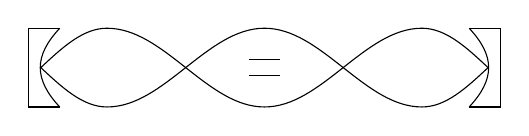
\begin{tikzpicture}[xscale=2]
                \draw (0, 1) -- (0, 0);
                \draw (0, 1) -- (0.2, 1);
                \draw (0, 0) -- (0.2, 0);
                \draw (0.2, 0) to [out=-245, in=245] (0.2, 1);

                \draw (3, 1) -- (3, 0);
                \draw (2.8, 1) -- (3, 1);
                \draw (2.8, 0) -- (3, 0);
                \draw (2.8, 0) to [out=-295, in=295] (2.8, 1);

                \draw (0.08, 0.5) sin (0.5, 1) cos (1, 0.5) sin (1.5, 0) cos (2, 0.5) sin (2.5, 1) cos (2.92, 0.5);

                \draw (0.08, 0.5) sin (0.5, 0) cos (1, 0.5) sin (1.5, 1) cos (2, 0.5) sin (2.5, 0) cos (2.92, 0.5);

                \draw (1.4, 0.4) -- (1.6, 0.4);
                \draw (1.4, 0.6) -- (1.6, 0.6);
        \end{tikzpicture}
    \end{center}
    Single cavity mode interacting with two level system in the RWA.
    Add coherent drive, dissipation via cavity loss $\kappa$ \& 
    spontaneous emission rate $\gamma$
    \begin{block}{Interaction Hamiltonian}
        $
        \mathscr{H} = \hbar \delta_{cd} a^\dagger a + 
        \hbar \delta_{qd}\sigma_+ \sigma_- + 
        \hbar g ( a \sigma_+ + a^\dagger \sigma_- ) + 
        \hbar \xi (a + a^\dagger) 
        $
    \end{block}
    \begin{block}{Master Equation}
        $
        \dot{\rho_S} = \frac{i}{\hbar} [ \mathscr{H}, \rho_S ] +
        \mathscr{L}_{\gamma} [\rho_S] + \mathscr{L}_{\kappa}[ \rho_S ]
        $
    \end{block}
\end{frame}
%----------------------------------------------------------------------
% Notes
    \note{
      \begin{itemize}
        \item no hats on operators.
        \item without cavity g becomes rabi frequency
        \item L are lindblad dissipators.
        \item In interaction picture, in the Markow approximation,
                with RWA, drive is coherent.
      \end{itemize}
        }
%----------------------------------------------------------------------
\begin{frame}
    \frametitle{Methods}
    \begin{columns}[T]
        \begin{column}{0.5\linewidth}
            \begin{block}{Meanfield}
\begin{align}
&\frac{d \alpha}{dt} = -(\kappa -i \Delta \omega) \alpha-ig \beta\\ 
&\frac{d \beta}{dt} = i \Delta \omega \beta +ig \alpha \zeta\\ 
&\frac{d \zeta}{dt} = 2 i g(\alpha^* \beta -\alpha \beta^*)
\end{align}
            \end{block}
        \end{column}
        \begin{column}{0.5\linewidth}
            \begin{block}{Master Equation}
\begin{align} 
    \mathscr{H} = &\hbar \delta (a^\dagger a + 
    \sigma_z) + \\ \nonumber
    &\hbar g ( a \sigma_+ + a^\dagger \sigma_- ) + \\ \nonumber
    &\hbar \xi (a + a^\dagger) 
\end{align}
            \end{block}
        \end{column}
    \end{columns}
\end{frame}
%----------------------------------------------------------------------
% Notes
    \note{
      \begin{itemize}
        \item Methods 
        \item Mean field eqs don't have gamma in them (they should)
      \end{itemize}
        }
%----------------------------------------------------------------------
\begin{frame}
    \begin{block}{Resonant}
        $
        \delta_{cq} = 0 \approx \delta_{cd}
        $
        \footfullcite{Alsing1990}
        \footfullcite{Carmichael2015}
    \end{block}
\end{frame}
%----------------------------------------------------------------------
% Notes
    \note{
      \begin{itemize}
        \item cd-det is only close to zero
        \item Alsing, Carmichael, Savage
      \end{itemize}
    }
%---------------------------------------------------------------------
\begin{frame}
  \includepdf{resonant.pdf}
\end{frame}
%---------------------------------------------------------------------
    % Notes
    \note{
      \begin{itemize}
        \item photon blockade - single photon dresses qubit, shifts
                resonance.
        \item Two types of bistability, phase - increasing drive
                amplitude - increase detuning
      \end{itemize}
        }
%----------------------------------------------------------------------
\begin{frame}
    \begin{block}{Dispersive}
        $
        \gamma \ll \kappa \ll g \ll \delta_{cq} \ll \omega_c
        $
        \footfullcite{Bishop2010}
    \end{block}
\end{frame}
%----------------------------------------------------------------------
% Notes
    \note{
      \begin{itemize}
        \item Hierarchy of scales 
      \end{itemize}
        }
%----------------------------------------------------------------------
\begin{frame}
    \frametitle{Why the dispersive regime?}
    \begin{block}{Qubit Readout \& Control}
        \begin{itemize}
            \item We can read out the state of the qubit 
                    without destroying it\footfullcite{Blais2004a}. 
            \item In the dispersive regime the qubit pulls the 
                    cavity frequency up or down based on its state.
            \item Driving the cavity at what was cavity 
                    resonance encodes the qubit superposition 
                    in the transmitted photons. 
            \item Driving the qubit can be used to coherently 
                    control the qubit state. 
        \end{itemize}
    \end{block}
\end{frame}
%----------------------------------------------------------------------
% Notes
    \note{
      \begin{itemize}
        \item Readout and Control
        \item Similar scheme for resonant case
      \end{itemize}
        }
%----------------------------------------------------------------------
\begin{frame}
    \frametitle{Effect of the detuned qubit}
    \begin{block}{Exact Hamiltonian}
        $
        \mathscr{H} = \hbar \delta_{cd} a^\dagger a + 
        \hbar \delta_{qd}\sigma_+ \sigma_- + 
        \hbar g ( a \sigma_+ + a^\dagger \sigma_- ) 
        +\hbar \xi (a+a^\dagger)
        $
    \end{block}
    \begin{block}{Dispersive Hamiltonian}
    We unitarily decouple the qubit and cavity 
    and expand to second order in $\frac{g}{\delta_{cq}}$. Defining 
    $\chi = \frac{g^2}{\delta_{cq}}$
    $\mathscr{A}_{JC} = \frac{g^2}{\delta_{cq}^3}$, 
    and freezing the qubit degree of freedom 
    $\sigma_z = -1$
    \begin{align}
    U\mathscr{H}U ^ \dagger \approx& 
         \left(\omega_c - \chi\right) a ^ \dagger a
        + \mathscr{A}_{JC}\left(a^\dagger a\right)^2
        + \xi ( a + a^\dagger ) \\
    \mathscr{H}_{duffing} &= \omega_c' a^\dagger a 
        + \mathscr{A} \left(a^\dagger a\right)^2 
        + \xi'\left(a+a^\dagger\right)
    \end{align} 
    The qubit pulls the cavity frequency. 
    To second order there is excitation dependent 
    duffing nonlinearity.
    \end{block}
\end{frame}
%----------------------------------------------------------------------
% Notes
\note{
    \begin{equation}
        \mathscr{H} = \omega_c a^ \dagger a
        + (\omega_c - \Delta)) \sigma_z/2
        + \xi / \sqrt{2} (a + a ^ \dagger ) \cos( \omega_d t )
    \end{equation}
    where
    \begin{equation}
        \Delta = \sqrt{\delta_{cq}^2 + 4g^2 N}
    \end{equation}
    \begin{equation}
        \mathscr{H} = (\omega_c
        - \frac{4g^2\sigma_z}{\delta_{cq}}) a ^ \dagger a
        + (\omega_q/2 - \frac{2g^2}{\delta_{cq}} (\sigma_z + 1))\sigma_z
        + \xi/\sqrt{2} (a + a^\dagger)\cos(\omega_d t)
    \end{equation}
    \begin{align}
        \mathscr{H} &= \omega_c a ^ \dagger a
        + (\omega_q/2) \sigma_z
        +  \xi/\sqrt{2} (a + a^\dagger) \cos(\omega_d t)\\
        &- \frac{4g^2}{\delta_{cq}}\left(a^\dagger a 
        +  \frac{\sigma_z}{2} + \frac{1}{2}\right)\sigma_z\\
        &- \frac{g^4}{\delta_{cq}^3}\left(
        \left(a^\dagger a\right)^2
        + \left(\frac{\sigma_z}{2}\right)^2
        + \left(\frac{1}{2}\right)^2
        + \frac{1}{2} \left(
                        a^\dagger a \sigma_z + \sigma_z a^\dagger a
                      \right)
        + a^\dagger a + \frac{\sigma_z}{2}
        \right)
        \sigma_z
    \end{align}
  }
%------------------------------------------------------------------------
\begin{frame}
    \begin{center}
        \includegraphics[scale=0.5]{leaf.png}
    \end{center}
    \begin{itemize}
        \item Unlike the Duffing nonlinearity 
            \footfullcite{Drummond1979},
            the nonperturbative JC nonlinearity softens with 
            increasing drive
            \footfullcite{Bishop2010}.
        \item The qubit participates in the system dynamics
    \end{itemize}
\end{frame}
%----------------------------------------------------------------------
% Notes
    \note{
      \begin{itemize}
        \item Duffing bistability region gets larger with 
                increasing drive? 
      \end{itemize}
        }
%----------------------------------------------------------------------
\begin{frame}
    \includepdf{dispersive.pdf}
\end{frame}
%----------------------------------------------------------------------
% Notes
    \note{
      \begin{itemize}
        \item Switching rates
        \item entanglement
      \end{itemize}
        }
%----------------------------------------------------------------------
\begin{frame}
    \printbibliography\
\end{frame}
%----------------------------------------------------------------------
\end{document}
